\section{Experimental Method}

\subsection{Fabrication and imaging}

Four distinct two-dimensional arrays of nanoscale geometries were fabricated using a FEI Helios G2 DualBeam FIB. The arrays were patterned so that each grid contained polygons of increasing size, and an increasing number of sides, from triangles to nonagons.
Material was selectively removed from the regions surrounding the patterned shapes, resulting in raised features relative to the milled background.

The structures were milled into a SiN TEM membrane grid, consisting of a 30 nm thick Si$_{3}$N$_{4}$ supporting layer, coated with) a 20 nm deposited film of permalloy (Ni$_{80}$Fe$_{20}$) and protected by a 2 nm thick Al capping layer. This was done using an ion beam ($ \mathrm{Ga^{+}} $) current of 48 $p$A, an acceleration voltage of 30 $k$V, a dwell time of $1\,\mu\text{s}$ and $203$ passes.
The TEM measurements were performed using a JEOL JEM-2100F in scanning mode, equipped with a field emission gun (FEG), and operated at an accelerating voltage of 200 kV. STEM differential phase contrast (STEM-DPC) 4D datasets were acquired, using a tilt of $t_x =$ -0.1 $mRad$  and $t_y =$ 1.6 $mRad$ in the x and y direction respectively.

\subsection{Data processing}
%\subsubsection{Data processing}
%The data was then processed using  HyperSpy version 2.3.0 \cite{de_la_pena_2016_hyperspy} on the IDUN cluster \cite{sjalander+:2019epic} to the sheer volume of data produced by the microscope (256$\times$256 $\times$ 256$\times$64). First to convert the data into an initial sample image which the magnetic data was later layered onto, the diffraction data was summed up for each probe position giving a 256$\times$256 image. For the magnetic contrast we first calculate the displacement of  center of the diffraction data on the 256$\times$64 sensor, converting the data into 256$\times$256$\times$2 array. Additionally we subtract a linear plane to compensate for the fact the the central beam is moving during the scan. Which then is layered onto the initial sample image.\textcolor{red}{Her burde Torbjørn beskrive hva han gjorde for å øke kontrasten}.\newline
%To calculate the "curl flux" we sliced the previous magnetic contrast array to isolate each polygon, and apply a mask to each of them slightly smaller than the polygon to reduce border effects. Resulting in only the magnetic displacement data for the polygon without the background noise around the polygon seen in Fig \ref{fig:STEM-DPC} resulting in an image, see Figure \ref{fig:hexagon}. After applying a mask to the data, we simply calculate the z-component of the curl using $\frac{\partial F_y}{\partial x} -\frac{\partial F_x}{\partial y}$, and divide by the number of pixels of the polygon.
The data was processed using Python, namely the Hyperspy package version 2.3.0 \cite{de_la_pena_2016_hyperspy} on the IDUN cluster \cite{sjalander+:2019epic} due to the sheer volume of data produced by the microscope (256$\times$256 $\times$ 256$\times$64). First, to convert the data into an initial sample image which the magnetic data was later layered onto, the diffraction data was summed up for each probe position, giving a 256$\times$256 image. For the magnetic contrast we first calculate the displacement of the center of the diffraction data on the 256$\times$64 sensor, converting the data into 256$\times$256$\times$2 array. Additionally, we subtract a linear plane to compensate for the fact the the central beam is moving during the scan. The resulting array is then layered onto the initial sample image. To enhance the visibility of significant data we used a virtual bright field (a sum showing sample geometry) as a mask. We applied the mask through the skimage.morphology.binary\_dilation and binary\_erosion functions.

\begin{figure}[H]
    \centering
    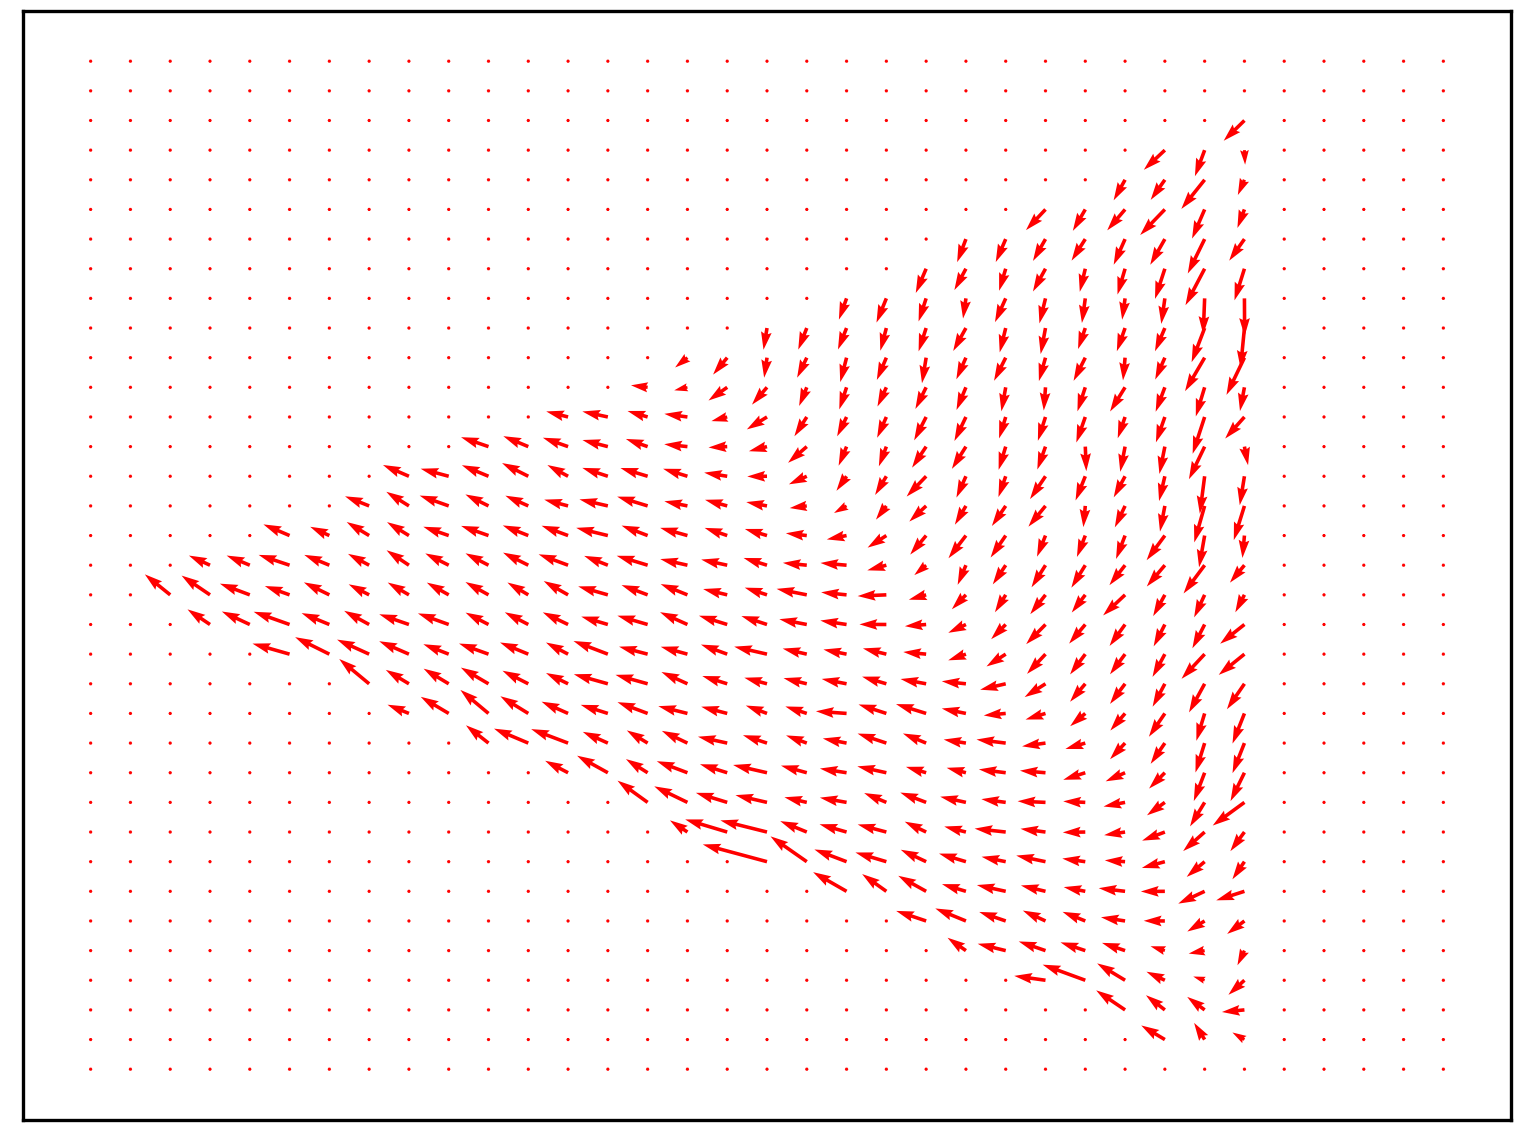
\includegraphics[width=1\columnwidth]{Images/triangle.png}
    \caption{Graphical representation of the magnetic field for the second largest triangular structure.}
    \label{fig:triangle}
\end{figure}
To calculate the ``curl flux'', we sliced the previous magnetic contrast array to isolate each polygon, and applied a slightly smaller mask than the polygon itself to each polygon to minimize border effects caused by image quality. %This gives us only the magnetic displacement data for the polygon without the interference of background noise seen in Figure \ref{fig:STEM-DPC} resulting in an image seen Figure \ref{fig:hexagon}.
After applying a mask to the data, we simply calculated the z-component of the curl using $\frac{\partial F_y}{\partial x} -\frac{\partial F_x}{\partial y}$. %\textcolor{red}{we now have a total curl for each figure, corresponding to the average curl per pixel, normalized with respect to its area}



For each pixel, the curl magnitude was calculated based on the magnetic field in the structure, as seen in Figure \ref{fig:triangle}, and the total curl was summed and then divided by the polygon’s pixel count to account for variations in shape size.

\begin{figure}[H]
    \centering
    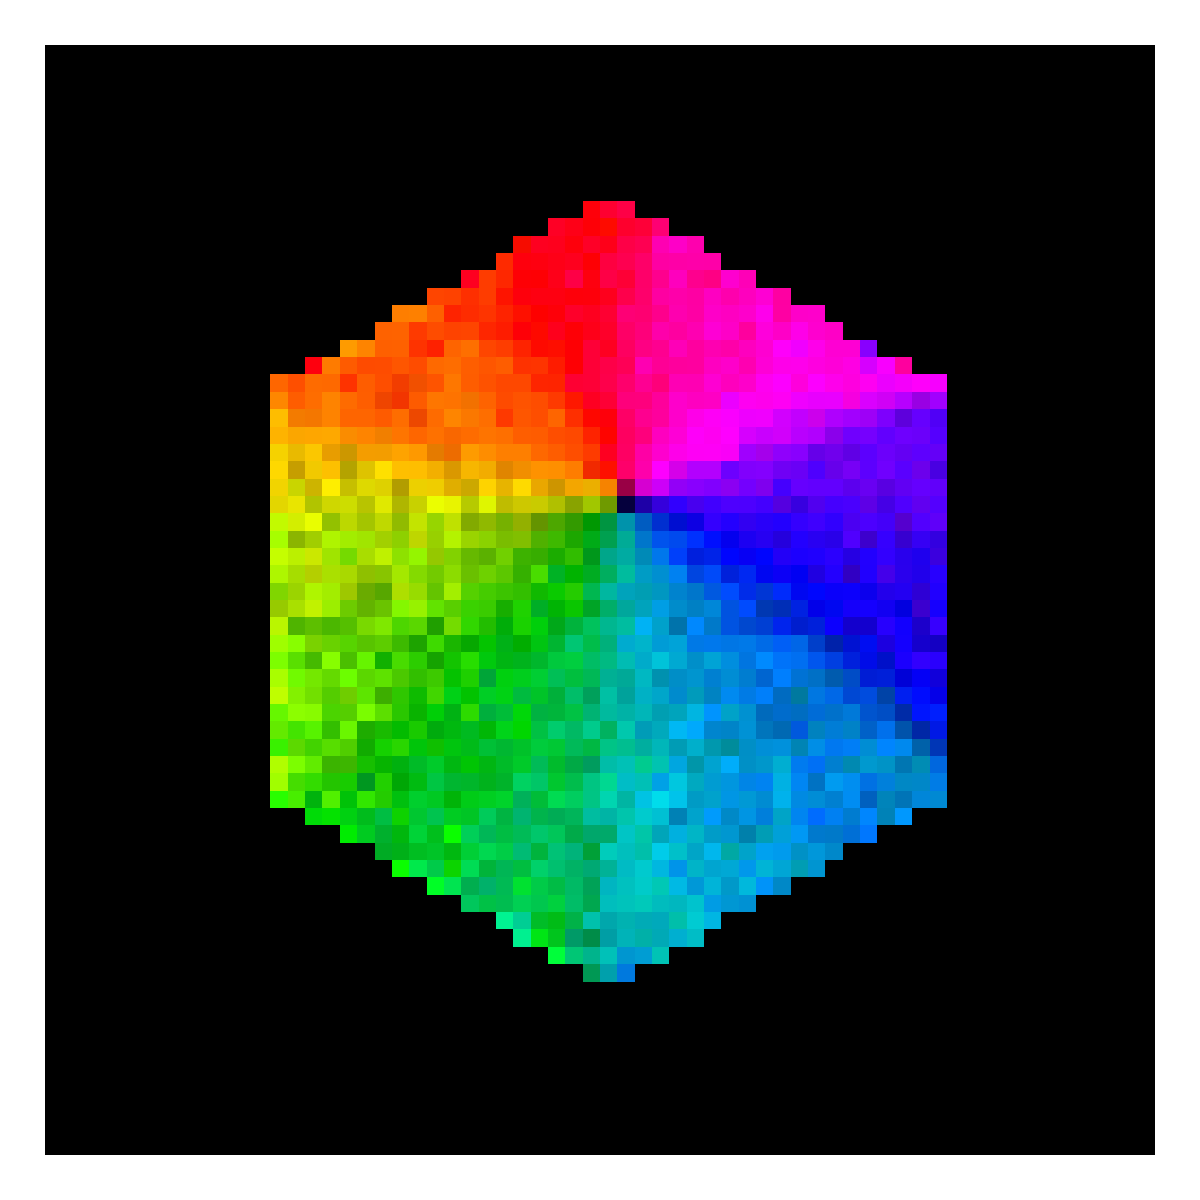
\includegraphics[width=0.4\columnwidth]{Images/hexagon.png}
    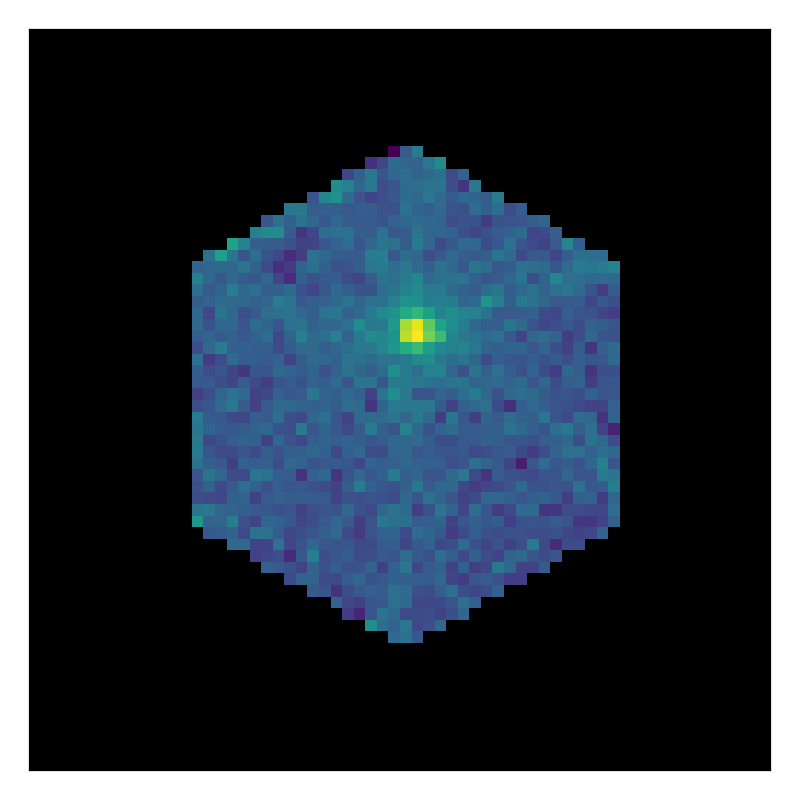
\includegraphics[width=0.4\columnwidth]{Images/raw_hexagon.png}
    \caption{Masked hexagon (left) used to calculate curl flux, and the resulting curl image (right).}
    \label{fig:hexagon}
\end{figure}

The resulting curl was plotted as a function of the number of polygon sides. Polygons of the same order of magnitude within a few hundred nanometers were analyzed and compared, from triangles to nonagons. This process was repeated three times for polygons of three different orders of magnitude. Approximately 900, 600 and 400 nm in radii.